% Latex template: mahmoud.s.fahmy@students.kasralainy.edu.eg
% For more details: https://www.sharelatex.com/learn/Beamer

\documentclass{beamer}					% Document class
\geometry{papersize={15cm,10cm}}

%\setbeamertemplate{footline}[text line]{%
%  \parbox{\linewidth}{\vspace*{-8pt}\hfill\hfill\insertpagenumber}}
\setbeamertemplate{navigation symbols}{}

\usepackage[english]{babel}				% Set language
\usepackage[utf8x]{inputenc}			% Set encoding

\mode<presentation>						% Set options
{
  \usetheme{default}					% Set theme
  \usecolortheme{default} 				% Set colors
  \usefonttheme{default}  				% Set font theme
  \setbeamertemplate{caption}[numbered]	% Set caption to be numbered
}

% Uncomment this to have the outline at the beginning of each section highlighted.
%\AtBeginSection[]
%{
%  \begin{frame}{Outline}
%    \tableofcontents[currentsection]
%  \end{frame}
\usepackage{graphicx}					% For including figures
\usepackage{booktabs}					% For table rules
\usepackage{hyperref}	
\usepackage{tikz-network}				% For cross-referencing
\usepackage[absolute,overlay]{textpos}
\usepackage{bm}
\usepackage[font=small,labelfont=bf]{caption}				% For cross-referencing
\usepackage{comment}
\usepackage{braket}
\usepackage{animate}

\title{Diffusion based generative models for modern fluorescence microscopy}	% Presentation title
\author{Clayton W. Seitz, Ph.D.}								% Presentation author
\date{\today}									% Today's date	

\AtBeginSection[]{
  \begin{frame}
  \vfill
  \centering
  \begin{beamercolorbox}[sep=8pt,center,shadow=true,rounded=true]{title}
    \usebeamerfont{title}\insertsectionhead\par%
  \end{beamercolorbox}
  \vfill
  \end{frame}
}

\begin{document}

% Title page
% This page includes the informations defined earlier including title, author/s, affiliation/s and the date
\begin{frame}
  \titlepage
\end{frame}

\begin{frame}{Outline of the talk}
    \tableofcontents
\end{frame}



% The following is the most frequently used slide types in beamer
% The slide structure is as follows:
%
%\begin{frame}{<slide-title>}
%	<content>
%\end{frame}

\setbeamertemplate{footline}{
    \hbox{%
    \begin{beamercolorbox}[wd=\paperwidth,ht=1.0ex,dp=1.5ex,leftskip=2ex,rightskip=2ex]{page ooter}%
        \footnotesize
        \usebeamerfont{title in head/foot}%
        Introduction to fluorescence nanoscopy \hfill
            %\insertsection \hfill
        \insertframenumber{} / \inserttotalframenumber
    \end{beamercolorbox}}%
}

\begin{frame}{Research Interests}
\begin{textblock*}{6cm}(3.0cm,1.5cm)
\includegraphics[width=6cm]{../../postdoc/sartorius/media/Me.png}
\end{textblock*}


\begin{textblock*}{10cm}(1.0cm,7cm)
\begin{itemize}
\item Machine learning methods for enhanced light microscopy
\item Quantitative single molecule localization microscopy 
\item Generative models, theory of deep learning
\end{itemize}
\end{textblock*}

\end{frame}

\section{Live cell super resolution microscopy}

\begin{frame}{A live cell fluorescence imaging zoo}

\end{frame}

\begin{frame}{The inherent tradeoffs of fluorescence microscopy}
\begin{textblock*}{12cm}(1.0cm,1.5cm)
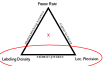
\includegraphics[width=12cm]{../../postdoc/sartorius/media/Tradeoff.png}
\emph{Courtesy of Chowdhury lab at UT Austin}
\end{textblock*}
\begin{textblock*}{12cm}(1.0cm,6.0cm)
\begin{itemize}
\item Ex. increase in resolution is often accompanied by loss of imaging speed
\item Computational methods such as AI/ML algorithms can help find a superior balance
\end{itemize}
\end{textblock*}
\end{frame}


\begin{frame}{Single molecule localization microscopy (SMLM)}

\begin{textblock*}{10cm}(2.0cm,2.0cm)
\animategraphics[width=10cm,autoplay,loop]{60}{../../postdoc/sartorius/media/Tower/storm-animation-}{1}{40}
\end{textblock*}

\begin{textblock*}{10cm}(2.0cm, 7.0cm)
SMLM is all about \emph{control} of the fluorescence 
\end{textblock*}

\end{frame}

\begin{frame}{Single molecule localization microscopy (SMLM)}

\begin{textblock*}{5cm}(2.0cm,3.0cm)
\includegraphics[width=5cm]{../../postdoc/sartorius/media/STORM.png}
\end{textblock*}

\begin{textblock*}{4cm}(9.0cm, 3.0cm)
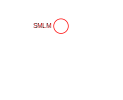
\includegraphics[width=4cm]{../../postdoc/sartorius/media/Tradeoff-SMLM.png}
\end{textblock*}

\begin{textblock*}{10cm}(1.5cm,8.0cm)
\begin{itemize}
\item SMLM techniques can achieve 10nm resolutions (20x higher than diffraction limit) 
\end{itemize}
\end{textblock*}

\end{frame}

\begin{frame}{Single molecule localization microscopy}
\begin{textblock*}{9cm}(0.5cm,1.5cm)
\includegraphics[width=\textwidth]{../../phd/dissertation/dissertation/media/Intro-Cropped.png}
\end{textblock*}
\begin{textblock*}{5cm}(9.5cm,1.5cm)
\animategraphics[width=5cm,autoplay,loop]{60}{../../phd/dissertation/dissertation/media/storm-animation/storm-animation-}{1}{100}
\end{textblock*}
\begin{textblock*}{15cm}(0.5cm,7.5cm)
\begin{itemize}
\item STORM and similar nanoscopy techniques are limited by localization precision
\item Higher lateral/axial resolution than other methods (e.g., SIM,STED,Confocal)
\item Poor time resolution
\end{itemize}
\end{textblock*}
\end{frame}

\begin{frame}{Stochastic optical reconstruction microscopy (STORM)}
\begin{textblock*}{9cm}(0.5cm,1.5cm)
\includegraphics[width=\textwidth]{../../phd/dissertation/dissertation/media/Intro-Cropped.png}
\end{textblock*}
\begin{textblock*}{5cm}(9.5cm,1.5cm)
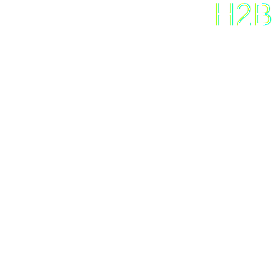
\includegraphics[width=\textwidth]{../../phd/dissertation/dissertation/media/STORM-Example.png}
\end{textblock*}
\begin{textblock*}{15cm}(0.5cm,7.5cm)
\begin{itemize}
\item STORM and similar nanoscopy techniques are limited by localization precision
\item Higher lateral/axial resolution than other methods (e.g., SIM,STED,Confocal)
\item Poor time resolution
\end{itemize}
\end{textblock*}
\end{frame}


\begin{frame}{Nanoscopy by localizing isolated fluorescent emitters}
\begin{itemize}
\item Modeling the point spread function permits sub-pixel localization 
\end{itemize}
\begin{textblock*}{8cm}(6.5cm,3.0cm)
\includegraphics[width=\textwidth]{../../phd/dissertation/dissertation/media/Model.png}
\end{textblock*}

\begin{textblock*}{2cm}(1cm,2.0cm)
\begin{align*}
\mu_{k} &= i_{0}\int\int O(u,v)dudv + \textcolor{pink}{\lambda}\\
i_{0} &= g_{k}\textcolor{red}{\eta} \textcolor{cyan}{\zeta}\textcolor{blue}{\Delta} 
\\
g_{k} &- \mathrm{pixel\; gain}\\
\textcolor{red}{\eta} &- \mathrm{quantum\; efficiency}\\
\textcolor{cyan}{\zeta} &- \mathrm{photon\; emission\; rate}\\
\textcolor{blue}{\Delta} &- \mathrm{exposure\; time}\\
\textcolor{pink}{\lambda} &- \mathrm{background \; rate}
\end{align*}
\end{textblock*}

\vspace{2in}

Maximum likelihood localization:

\begin{equation*}
\theta^{*} = \underset{\theta}{\mathrm{argmax}}\prod_{k}p(\bold{x}_{k}|\theta)= \underset{\theta}{\mathrm{argmin}}-\sum_{k}\log p(\bold{x}_{k}|\theta)
\end{equation*}

\end{frame}


\begin{frame}{Tracking chromatin loci photoactivated localization microscopy}
\begin{textblock*}{12cm}(2.0cm,1.5cm)
\includegraphics[width=12cm]{../../postdoc/sartorius/media/DOE.png}
Locatelli, Seitz et al. PNAS \textbf{29} (2022)
\end{textblock*}
\end{frame}

\begin{frame}{Tracking chromatin loci photoactivated localization microscopy}
\begin{textblock*}{12cm}(2.0cm,1.5cm)
\includegraphics[width=12cm]{../../postdoc/sartorius/media/Bleo.png}
Locatelli, Seitz et al. PNAS \textbf{29} (2022)
\end{textblock*}
\end{frame}


\begin{frame}{Analyzing the structure nucleosome nanodomains with SMLM}
\begin{textblock*}{10cm}(2.0cm,1.5cm)
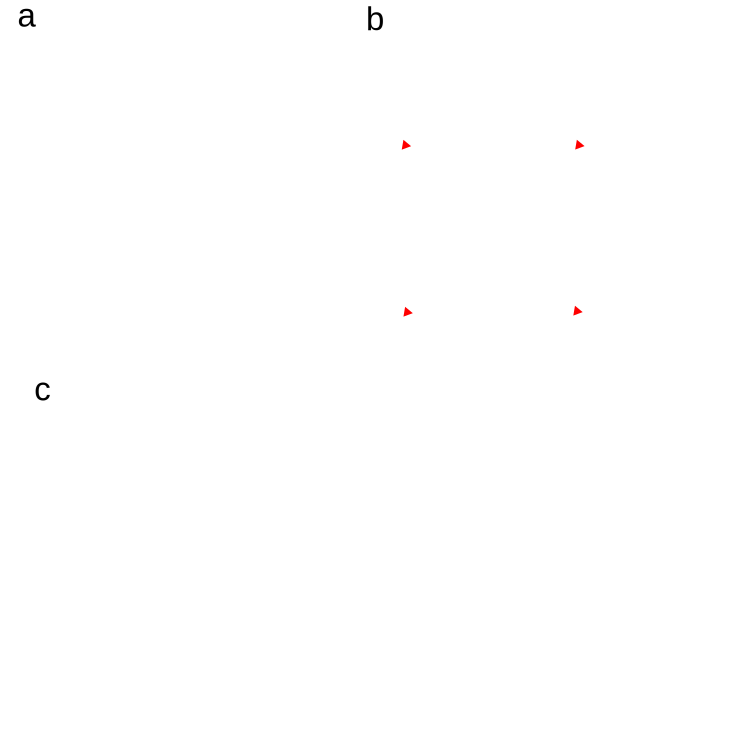
\includegraphics[width=10cm]{../../phd/brd4/brd4/media/Figure-2.png}
Seitz et al. bioRxiv, Cells, In Review (2025)
\end{textblock*}

\begin{textblock*}{13cm}(1.0cm,8.0cm)
\begin{itemize}
\item H2B is densely labeled for super-resolution imaging
\item BRD4 chromatin binding activity controls nanodomain density
\end{itemize}
\end{textblock*}
\end{frame}


\begin{frame}{Quantitative SMLM by measuring the photon counting histogram}
%\begin{textblock*}{13cm}(1.0cm,1.0cm)
\includegraphics[width=10cm]{../../postdoc/sartorius/media/SPAD512.png}
%\end{textblock*}
\end{frame}

\begin{frame}{Quantitative SMLM by measuring the photon counting histogram}
%\begin{textblock*}{13cm}(1.0cm,1.0cm)
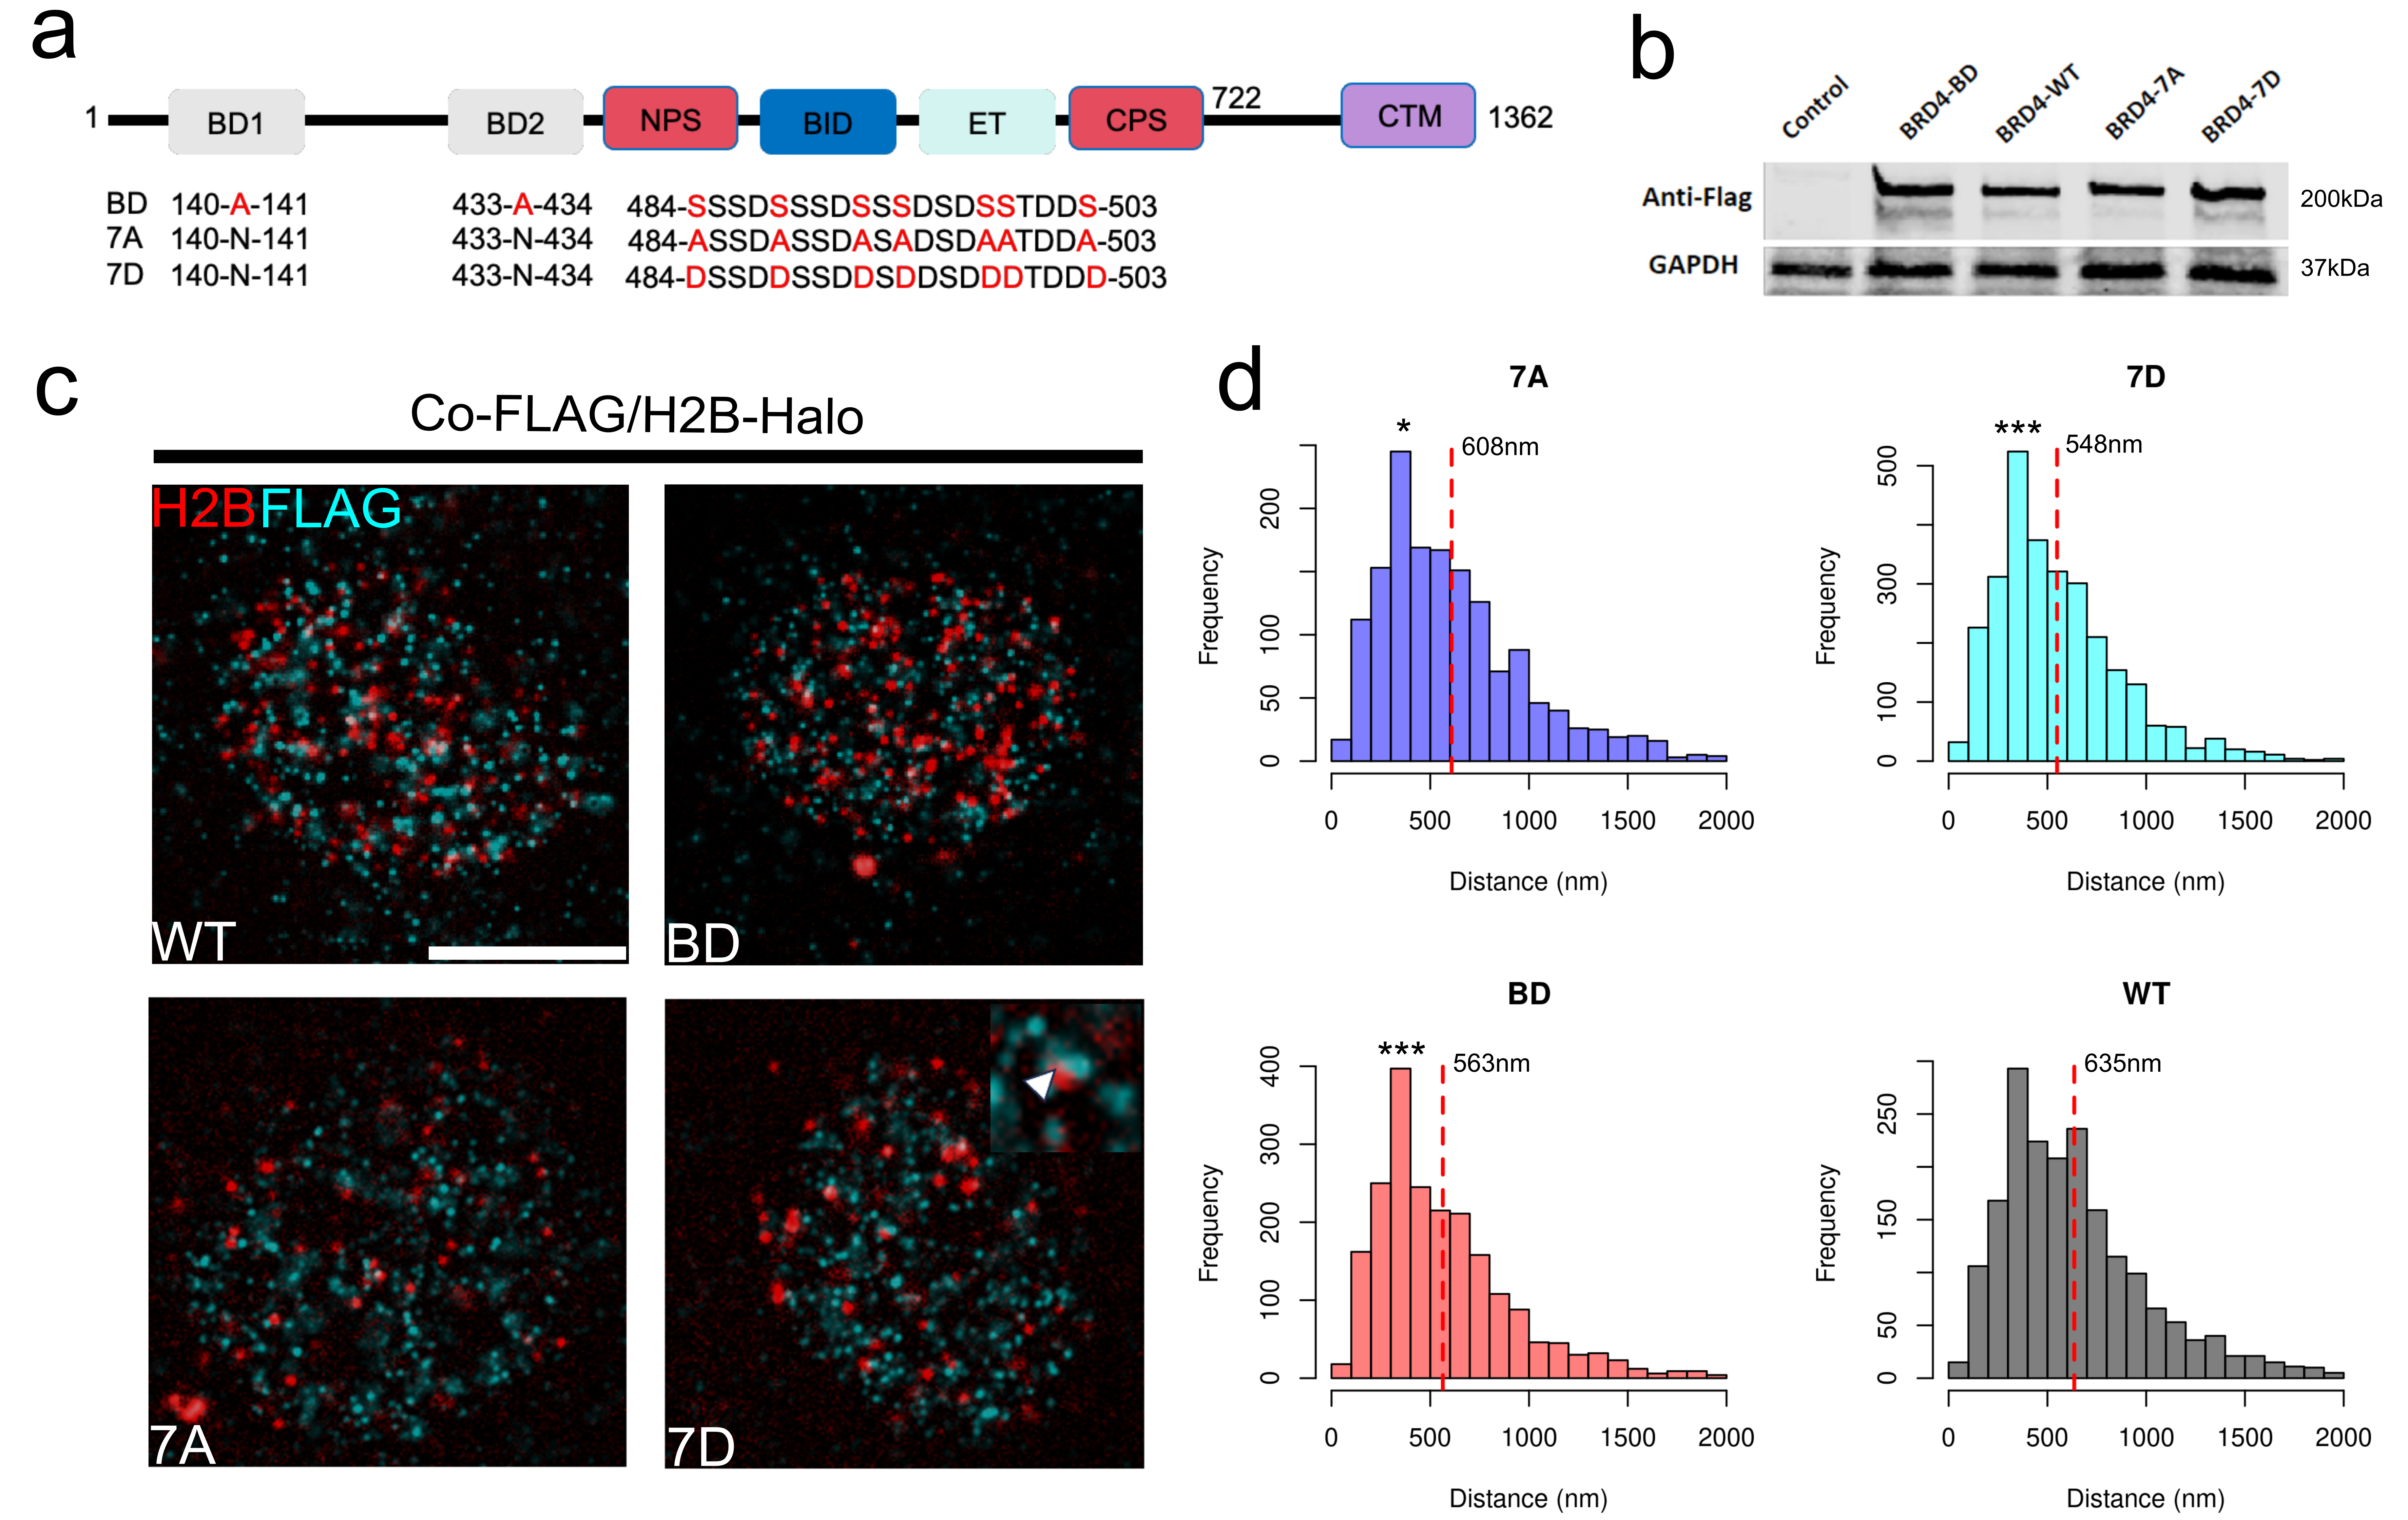
\includegraphics[width=12cm]{../../phd/spad/spad/media/Figure-0.png}
\\Seitz et al. Communications Physics, In Review (2025)
%\end{textblock*}
\end{frame}



\setbeamertemplate{footline}{
    \hbox{%
    \begin{beamercolorbox}[wd=\paperwidth,ht=1.0ex,dp=1.5ex,leftskip=2ex,rightskip=2ex]{page ooter}%
        \footnotesize
        \usebeamerfont{title in head/foot}%
        Novel methods: probabilistic modeling approaches to fluorescence nanoscopy \hfill
            %\insertsection \hfill
        \insertframenumber{} / \inserttotalframenumber
    \end{beamercolorbox}}%
}

\section{Deep learning models for modern microscopy}


\begin{frame}{The inherent tradeoffs of fluorescence microscopy}
\begin{textblock*}{12cm}(1.0cm,1.5cm)
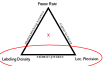
\includegraphics[width=12cm]{../../postdoc/sartorius/media/Tradeoff.png}
\emph{Courtesy of Chowdhury lab at UT Austin}
\end{textblock*}
\begin{textblock*}{12cm}(1.0cm,6.0cm)
\begin{itemize}
\item Ex. increase in resolution is often accompanied by loss of imaging speed
\item Computational methods such as AI/ML algorithms can help find a superior balance
\item Fluorescence microscopy is often not very quantitative (more on this later)
\end{itemize}
\end{textblock*}
\end{frame}

\begin{frame}{Deep learning based 3D reconstruction}
\begin{textblock*}{12cm}(2.0cm,1.5cm)
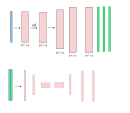
\includegraphics[width=12cm]{../../postdoc/sartorius/media/Arch.png}
\end{textblock*}
\end{frame}


\begin{frame}{Deep learning based 3D reconstruction}
\begin{textblock*}{12cm}(2.0cm,1.5cm)
\includegraphics[width=12cm]{../../postdoc/sartorius/media/UNET-1.png}
\end{textblock*}
\end{frame}

\begin{frame}{Deep learning based 3D reconstruction}
\begin{textblock*}{10cm}(2.0cm,1.5cm)
\includegraphics[width=10cm]{../../postdoc/sartorius/media/UNET-2.png}
\end{textblock*}
\end{frame}

\begin{frame}{Three-dimensional localization microscopy using deep learning}

\end{frame}

\begin{frame}{Deep learning based quantitative phase imaging}

\end{frame}

\begin{frame}{Resolution enhancement by deep learning}
\begin{center}
\includegraphics[width=10cm]{../../postdoc/sartorius/media/Deep-STORM.jpeg}
\\Nehme E. et al. Optica \textbf{5}, 458-464 (2018)
\vspace{0.5cm}
\begin{itemize}
\item Prediction of high resolution images from low resolution ones
\item Cannot report uncertainty, leading to overconfident results
\end{itemize}
\end{center}
\end{frame}

\begin{frame}{Inverse problems in microscopy are ill-posed}

\begin{itemize}
\item Inverse problems deal with the task of finding parameters of interest from observations
\item Inverse problems are usually \emph{ill-posed}
\item ``Ill-posed'' means that observations underdetermine the system
\end{itemize}



\end{frame}

\begin{frame}{Resolution enhancement with a diffusion model}
\begin{textblock*}{13cm}(0.5cm,1.5cm)
\begin{itemize}
\item Can sample from $p(\theta\lvert \boldsymbol{x})$ using a stochastic process called Langevin dynamics
\end{itemize}
\end{textblock*}
\begin{textblock*}{8cm}(3.5cm,2.0cm)
\animategraphics[width=8cm,autoplay,loop]{20}{../../phd/ddpm/ddpm/media/sampling/image-}{1}{100}
\end{textblock*}
\begin{textblock*}{14cm}(2.25cm,8.0cm)
\textcolor{red}{Drift} and \textcolor{blue}{diffusion}: 
$\theta_{t} = 
\overset{\mu}{\overbrace{\textcolor{red}{\theta_{t-1} - \frac{\beta}{2}\nabla f(\theta)}}} 
+ \textcolor{blue}{\sqrt{\beta}\xi} 
\;\;\; \xi \sim \mathcal{N}(0,I)$
\end{textblock*}
\end{frame}

\setbeamertemplate{footline}{
    \hbox{%
    \begin{beamercolorbox}[wd=\paperwidth,ht=1.0ex,dp=1.5ex,leftskip=2ex,rightskip=2ex]{page ooter}%
        \footnotesize
        \usebeamerfont{title in head/foot}%
        Novel methods: probabilistic modeling approaches to fluorescence nanoscopy \hfill
            %\insertsection \hfill
        \insertframenumber{} / \inserttotalframenumber
    \end{beamercolorbox}}%
}

\begin{frame}{Resolution enhancement with a diffusion model}

\begin{textblock*}{13cm}(1.0cm, 1.5cm)

\begin{itemize}
\item Task: infer a high resolution image $\bold{y}_0$ from low resolution $\bold{x}$
\item Drift is not available for image data, but can be learned from pairs $(\bold{x},\bold{y}_{0})$
\end{itemize}
\end{textblock*}

\begin{textblock*}{2cm}(6.0cm, 7.25cm)
\begin{equation*}
q(\bold{y}_{t}|\bold{y}_{t-1}) = \mathcal{N}\left(\sqrt{1-\beta_{t}}\bold{y}_{t-1},\beta_t I\right)
\end{equation*}
\end{textblock*}

\begin{textblock*}{12cm}(1.5cm, 4.25cm)

\includegraphics[width=12cm]{../../phd/ddpm/ddpm/media/ForwardBackward.png}
\end{textblock*}

\begin{textblock*}{2cm}(6.0cm, 3.0cm)
\begin{equation*}
p_{\psi}(\bold{y}_{t-1}|\bold{y}_{t},\bold{x}) = \mathcal{N}\left(\mu_{\psi},\beta_{t}I\right)
\end{equation*}

\end{textblock*}

\end{frame}

\begin{frame}{Resolution enhancement with a diffusion model}
\begin{textblock*}{9cm}(3.0cm, 2.0cm)
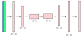
\includegraphics[width=9cm]{../../phd/ddpm/ddpm/media/DiffusionArch.png}
\end{textblock*}
\begin{textblock*}{2cm}(0.5cm, 3.0cm)
\includegraphics[width=2cm]{../../phd/dissertation/dissertation/media/diffusion_example/0_1_sr_79.png}
\end{textblock*}
\begin{textblock*}{2cm}(12.5cm, 3.0cm)
\includegraphics[width=2cm]{../../phd/dissertation/dissertation/media/diffusion_example/0_1_sr_99.png}
\end{textblock*}

\begin{textblock*}{13cm}(1.0cm, 6.5cm)
\begin{itemize}
\item A convolutional neural network $\psi$ estimates the drift $\mu_{\psi}$
\item Denoising step: $y_{t-1}\sim p_{\psi}(\bold{y}_{t-1}|\bold{y}_{t},\bold{x}) = \mathcal{N}\left(\mu_{\psi},\beta_{t}I\right)$
\end{itemize}
\end{textblock*}
\end{frame}

\begin{comment}
\begin{frame}{Bayesian image restoration with diffusion models}

\begin{textblock*}{2cm}(1.0cm, 1.0cm)
$\bold{x}$
\includegraphics[width=2cm]{../../phd/dissertation/dissertation/media/diffusion_example/Diffusion_lr-0.png}
\end{textblock*}
\begin{textblock*}{2cm}(4.0cm, 1.0cm)
$\bold{y}_{100}$
\includegraphics[width=2cm]{../../phd/dissertation/dissertation/media/diffusion_example/0_1_sr_1.png}
\end{textblock*}
\begin{textblock*}{2cm}(6.0cm, 1.0cm)
$\bold{y}_{80}$
\includegraphics[width=2cm]{../../phd/dissertation/dissertation/media/diffusion_example/0_1_sr_19.png}
\end{textblock*}
\begin{textblock*}{2cm}(8.0cm, 1.0cm)
$\bold{y}_{40}$
\includegraphics[width=2cm]{../../phd/dissertation/dissertation/media/diffusion_example/0_1_sr_39.png}
\end{textblock*}
\begin{textblock*}{2cm}(10.0cm,1.0cm)
$\bold{y}_{20}$
\includegraphics[width=2cm]{../../phd/dissertation/dissertation/media/diffusion_example/0_1_sr_79.png}
\end{textblock*}
\begin{textblock*}{2cm}(12.0cm, 1.0cm)
$\bold{y}_{0}$
\includegraphics[width=2cm]{../../phd/dissertation/dissertation/media/diffusion_example/0_1_sr_99.png}
\end{textblock*}

\begin{textblock*}{10cm}(2.0cm, 4.0cm)

\includegraphics[width=10cm]{../../phd/dissertation/dissertation/media/Bayes.png}
\end{textblock*}

\begin{textblock*}{12cm}(1.0cm, 7.5cm)
Estimation of pixel-wise uncertainty in the high resolution $\bold{y}$
\end{textblock*}


\end{frame}
\end{comment}

\begin{frame}{Super resolution with a diffusion model}
\begin{textblock*}{12cm}(2.0cm,1.5cm)
\includegraphics[width=12cm]{../../phd/ddpm/ddpm/media/Figure-2-1-crop.png}
\end{textblock*}
\end{frame}

\begin{frame}{Super resolution with a diffusion model}
\begin{textblock*}{12cm}(2.0cm,1.5cm)
\includegraphics[width=12cm]{../../postdoc/sartorius/media/Tubes-Crop.png}
\end{textblock*}
\end{frame}

\begin{frame}{Summary}

\end{frame}

\begin{frame}{Selected Publications}

\begin{itemize}

\item \textbf{C. Seitz}, D. Fu, M. Liu, H. Ma, and J. Liu. \textit{BRD4 phosphorylation regulates the structure of chromatin nanodomains}. In Review. Phys Rev Lett. 2024

\item \textbf{C. Seitz} and J. Liu. \textit{Uncertainty-aware localization microscopy by variational diffusion}. In Progress. 2024

\item \textbf{C. Seitz} and J. Liu. \textit{Quantum enhanced localization microscopy with a single photon avalanche diode array}. In Progress. 2024

\item M. Locatelli\textsuperscript{\textdagger}, J. Lawrimore\textsuperscript{\textdagger}, H. Lin\textsuperscript{\textdagger}, S. Sanaullah, \textbf{C. Seitz}, D. Segall, P. Kefer, S. Moreno Naike, B. Lietz, R. Anderson, J. Holmes, C. Yuan, G. Holzwarth, B. Kerry, J. Liu, K. Bonin, P. Vidi. \textit{DNA damage reduces heterogeneity and coherence of chromatin motions}. PNAS 12 July 2022; 119 (29): 1-11

\item M. Zhang, \textbf{C. Seitz}, G. Chang, F. Iqbal, H. Lin, and J. Liu \textit{A guide for single-particle chromatin tracking in live cell nuclei}. Cell Biology International 15 January 2022; 46 (5): 683-700


\end{itemize}
\end{frame}



\end{document}